\section{Results}

\subsection{Model Parameters and Metrics Analysis}

The Autoencoder-LSTM model was trained using a well-defined set of parameters and evaluated with comprehensive metrics. Below is an in-depth analysis of the results:

\subsubsection{Model Parameters}

\begin{itemize}
    \item \textbf{Cityname:} The model was trained to predict house prices for the city of Regina, focusing on regional trends and characteristics specific to this city.
    \item \textbf{Encoded Dimension (encoded\_dim):} The latent space of the autoencoder compresses the input features into 64 dimensions. This dimensionality is sufficient to capture essential patterns while reducing computational complexity.
    \item \textbf{Input Dimension (input\_dim):} The input data consists of 64 features after preprocessing, indicating the high-dimensional nature of the dataset.
    \item \textbf{Learning Rate:} The learning rate was set to 0.001, providing a balance between fast convergence and stable learning, as evidenced by the smooth decline in training and validation loss.
    \item \textbf{LSTM Hidden Dimension (lstm\_hidden\_dim):} The LSTM network utilized 128 hidden units, enabling it to capture temporal dependencies and long-term trends in the data effectively.
    \item \textbf{Number of LSTM Layers (lstm\_num\_layers):} The model employed a 2-layer LSTM architecture to balance model complexity and computational efficiency.
    \item \textbf{Number of Epochs (num\_epochs):} The model was trained for 50 epochs, sufficient for convergence without overfitting, as demonstrated by the stable loss metrics.
    \item \textbf{Output Dimension (output\_dim):} The output dimension was set to 1, as the task involves predicting a single target variable, the house price index.
\end{itemize}

\subsubsection{Model Metrics}

\begin{figure}[H]
    \centering
    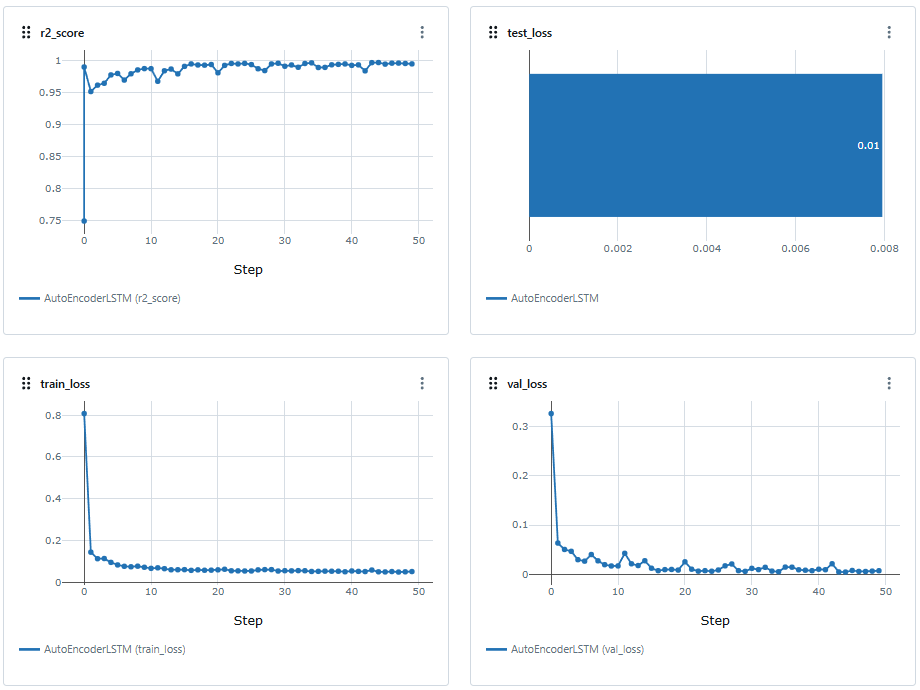
\includegraphics[width=0.8\textwidth]{images/results.png}
    \caption{Model performance metrics visualization.}
    \label{fig:results}
\end{figure}

\begin{itemize}
    \item \textbf{R² Score:} The model achieved an R² score of 0.994, indicating that it explains 99.4\% of the variance in the target variable. This high score highlights the model's ability to accurately predict house prices.
    \item \textbf{Test Loss (test\_loss):} The test loss was recorded as 0.00796, showcasing the model's strong generalization performance on unseen data.
    \item \textbf{Training Loss (train\_loss):} The final training loss was 0.0511, indicating that the model effectively minimized errors during training.
    \item \textbf{Validation Loss (val\_loss):} The validation loss stabilized at 0.00743, closely matching the test loss. This consistency reflects the model's robustness and absence of overfitting.
\end{itemize}

\subsection{Observations and Insights}

\begin{itemize}
    \item \textbf{Strong Generalization:} The close alignment of training, validation, and test losses demonstrates that the model generalizes well to unseen data. This indicates a good balance between underfitting and overfitting.
    \item \textbf{High Predictive Power:} The R² score close to 1 confirms that the model effectively captures patterns in the data and provides highly accurate predictions.
    \item \textbf{Efficiency of Hybrid Architecture:} The combination of autoencoders for dimensionality reduction and LSTMs for sequential modeling contributed to the model's strong performance. The autoencoder reduced noise and redundancy, while the LSTM layers captured temporal dependencies.
\end{itemize}

Overall, this project aims to leverage state-of-the-art machine learning techniques to predict house prices accurately, thereby empowering stakeholders with actionable insights and facilitating informed decision-making in the real estate sector. By addressing the challenges of house price prediction through advanced deep learning models, we aim to contribute to the advancement of real estate analytics and market intelligence.